\documentclass[10pt,a4paper]{article}
\usepackage[utf8]{inputenc}
\usepackage{amsmath}
\usepackage{amsthm}
\usepackage{amsfonts}
\usepackage{amssymb}
\usepackage{graphicx}
\usepackage{enumitem}
\usepackage[margin=1in]{geometry}

\newtheorem*{remark}{Remark}
\newtheorem{definition}{Definition}
\newtheorem{example}{Example}
\newtheorem{lemma}{Lemma}
\newtheorem{theorem}{Theorem}
\newtheorem{proposition}{Proposition}
\newtheorem{conjecture}{Conjecture}
\newtheorem{corollary}{Corollary}


\newcommand{\G}[2]{G_{\{#1,#2\}}}
\newcommand{\g}[2]{g_{\{#1,#2\}}}
\newcommand{\h}[2]{h_{#1}^{\{#2\}}}
\newcommand{\p}[2]{p_{(#1,#2)}}
\newcommand{\z}[1]{\bar{z}_{#1}}
\newcommand{\len}[1]{\left\lvert #1 \right\rvert}
\renewcommand{\i}{\mathrm{i}}
 
\title{Notes on triangulations of ideal hyperbolic $n$-gons}
\date{}

\begin{document}
\maketitle




\section{Notation}
\label{sec:notation}

\begin{figure}[h]
    \centering
    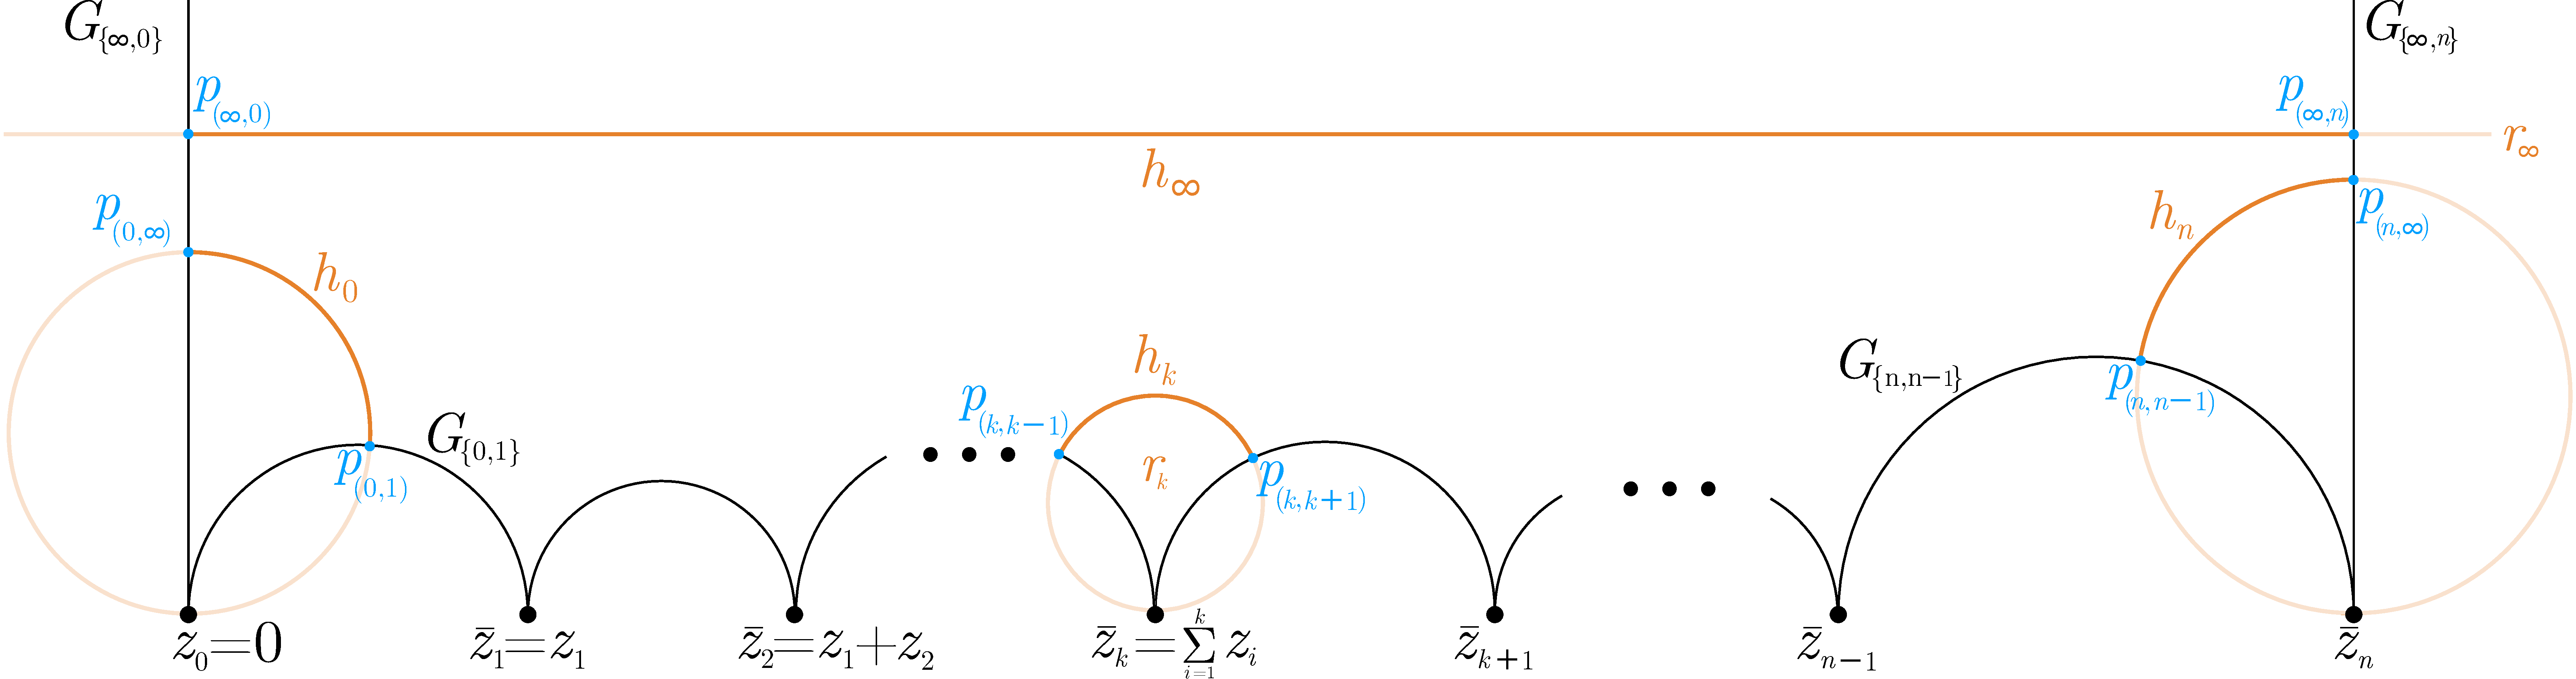
\includegraphics[width=1.0\textwidth]{notation2.pdf}
    \caption{Cartoon illustration of an ideal hyperbolic $(n+2)$-gon which highlights important elements: geodesics connecting adjacent ideal vertices $\z{k}$ (solid black) and horocycles, with radii $r_k$, centered at ideal vertices and horoarcs of  length $\alpha_k$ contained within the polygon (solid orange) with endpoints given by the points of intersection between the horocycles and geodesics (blue).}
    \label{fig:notation}
\end{figure}

Throughout these notes we will consider \textit{ideal hyperbolic} $(n+2)$-gons with vertices $\z{\infty} := \infty$ and $\z{k} \in \mathbb{R}, k = 0, \ldots, n$, with $\z{0} := 0, \bar{z}_{k} := \sum_{i=1}^{k} z_i$ and $z_i > 0$. We denote the geodesic connecting ideal vertices $\z{i} \neq \z{j}$ by $\G{i}{j}$. For example, the boundary of the polygon is the union of the geodesics $\G{k}{k \pm 1}$, for $0 < k < n$ together with $\G{0}{\infty}$ and $\G{n}{\infty}$.

We will refer to a horocycle, $H_k$, centered at $\z{k}$ ($k=0,\ldots, n$), by specifying its radius, $r_k$, which is equal to the diameter of the corresponding Euclidean circle that is tangent to the real line at $\z{k}$.  We reserve $r_{\infty} > 0$ for the height of the horizontal line defining the horocycle $H_{\infty}$ centered at $\z{\infty}$. We denote the ideal $(n+2)$-gon with vertices $\z{k}$ and horocycles with radii $r_k$, $k=0, \ldots, n, \infty$ by $\mathcal{P}((\z{k},r_k))$. 

The (non-ideal) point of intersection between the horocycle $H_k$ and the geodesic $\G{k}{j}$ will be denoted $\p{k}{j}$. Any two geodesics, $\G{k}{s}$ and $\G{k}{t}$, emanating from $\z{k}$, divide the Euclidean circle representing $H_k$ into two \textit{horoarcs}, only one or which has finite length. We denote this horoarc by $\h{k}{s,t}$. For example, the subset of $H_k$ that is contained within the polygon is the horoarc $h_{k} := \h{k}{k-1,k+1}$, for $0 < k < n $. If $k=0,n$ we similarly simplify notation and write $h_0 := \h{0}{1,\infty}$ and $h_n := \h{n}{n-1,\infty}$). See Fig.\ \ref{fig:notation} for an illustration of these variables. 

To simplify notation we will use $\len{\gamma(t)}$ to denote the length of a curve $\gamma: [0,1] \rightarrow \mathbb{H}$, as well as the usual absolute value of a real number.

\section{Mapping Merge Trees to Polygons}
\label{sec:mapmerge2poly}
In this section we justify limiting our focus to normal hyperbolic $n$-gons and establish their connection to rooted merge trees. We begin by describing a transformation mapping a rooted merge tree with $n-1$ leaves (and 1 root) to an ideal hyperbolic $n$-gon such that the tree is naturally associated with the Voronoi diagram of the vertices of the polygon. 

\begin{definition}
Given a real-valued function $f:K \rightarrow \mathbb{R}$ on a simplicial complex $K$ specified by linear interpolation of a scalar function defined on the vertices $K$ to its higher dimensional simplicies, we define the associated merge tree to be the quotient space $K/\sim$. Here for $x,y \in K$, $x \sim y$ if $f(x) = f(y)$, i.e. $x$ and $y$ belong to the same level set of $f$, and $x$ and $y$ belong to the same connected component of the sublevel set $f^{-1}(-\infty, f(x)]$.
\end{definition}

















 \section{Distance to Horocycles}
 \label{sec:dist2horos}

 \begin{figure}
     \centering
     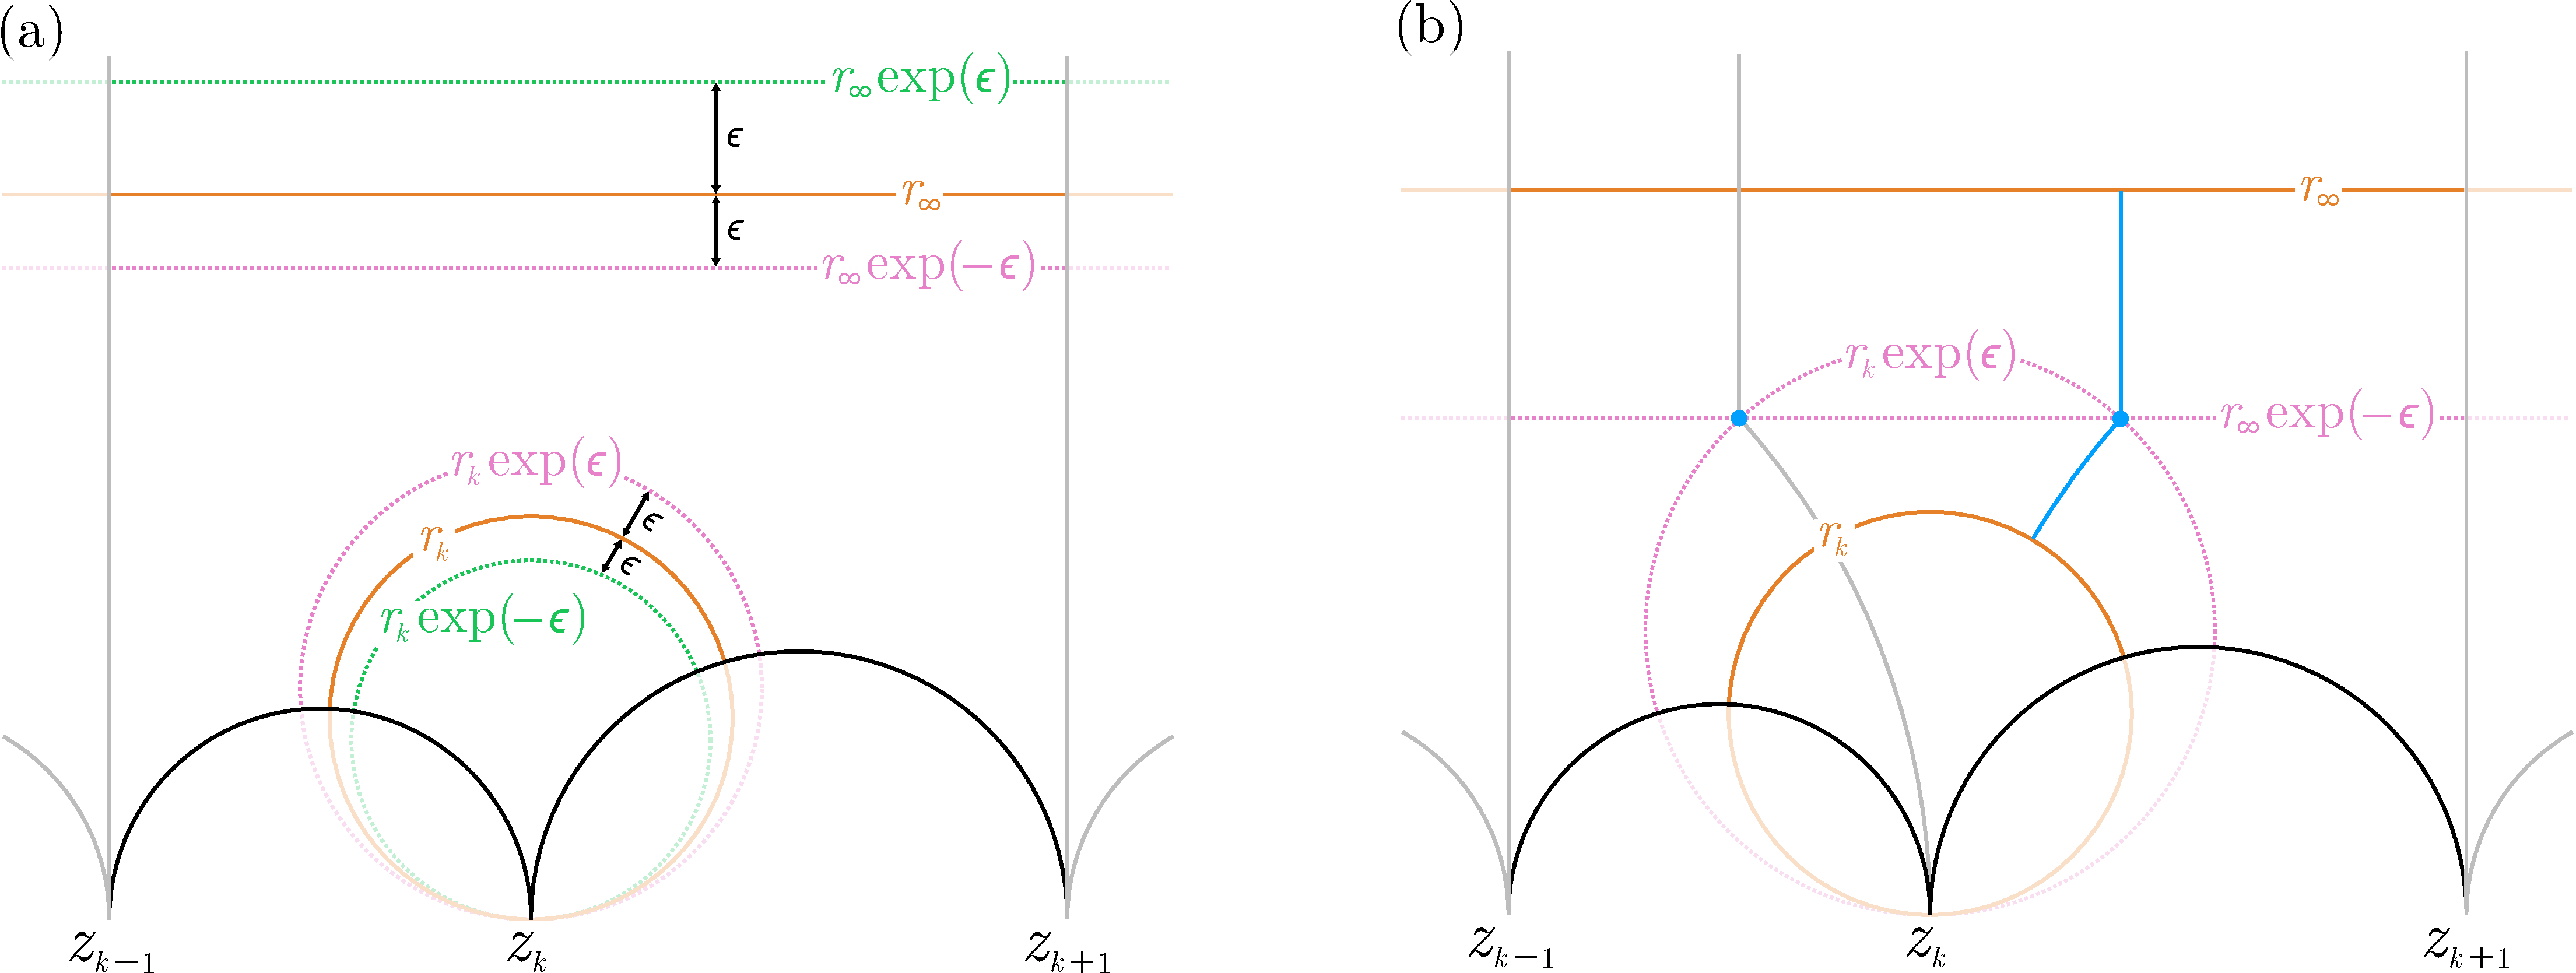
\includegraphics[width=1.0\textwidth]{concentric_horocycles.pdf}
     \caption{(a) Horocycles $H_{\infty}$ and $H_{k}$ (solid orange) with sets of points a distance $\epsilon$ (dotted green and pink) from each.  Colored curves are horocycles with centers at $\infty$ or $z_k$, labelled by their radii. (b) Horocycles $H_{\infty}$ and $H_{k}$ (solid orange) with intersecting sets of points a distance $\epsilon$ (dotted pink) from each. Two points an equal distance from both $H_{k}$ and $H_{\infty}$ are highlighted (blue dots), with distance determined by the equal-length geodesic segments (solid blue). Longer portions of the geodesics determining the distance from the highlighted points and each $H_{\infty}$ and $H_{k}$ are also indicated (solid gray).}
     \label{fig:concentric_horocycles}
 \end{figure}

 In order to define the Delaunay triangulation of a normal ideal hyperbolic $(n+3)$-gon, we must first understand the distances between points inside the polygon and the equal-area horocycles centered on its ideal vertices. Indeed, we will want the interior edges of a triangulation of the polygon to correspond to the geodesics connecting non-adjacent neighboring ideal vertices, where the neighbor relationship is determined by the adjacency of the Voronoi cells of the ideal vertices. As it happens, the boundary of the regions separating points that are closer to one or the other of two non-overlapping horocycles is always a geodesic in the hyperbolic plane.  As part of the proof we will derive formulas that allow us to compute these geodesics in the special case of non-overlapping horocycles with ideal centers $z_{\infty}, z_{-1}, z_0, z_1, \ldots, z_n$ that enclose regions within $\text{NIH}(z_1\ldots, z_n)$ of equal area.

 \begin{lemma}
 For $\epsilon > 0$ the set of points a distance $\epsilon$ to a horocycle $H$ with ideal center $x$ and radius $r$, consists of two concentric horocycles with center $x$ and radii $r \exp(\pm \epsilon)$.
 \label{lem:equidist2horo}
 \end{lemma}

 \begin{proof}
 First take $H$ to be centered at $x = \infty$, i.e. $H$ is a horizontal line segment at height $2r$.  The distance between a point $z = (a+ib)$ and the horocycle $H$, (denoted $d(z, H)$) is determined by the length of the vertical geodesic line segment connecting $z = (a+ib)$ and the point $a + i 2 r$; say this distance is $\epsilon$.  Since this holds for any $a$, the set of points which are a distance $\epsilon$ to $H$ form two concentric horocycles centered at $\infty$, namely the horizontal lines at heights $2r\exp(\epsilon)$ and $2r\exp(-\epsilon)$, as shown in Fig.\ \ref{fig:concentric_horocycles} (a). If the center of $H$ were any other ideal point $x$, we construct the isometry taking $\infty$ to $x$, and the horocycle of radius $r$ centered at $\infty$ (call it $H_{\infty}$) to the horocycle of radius $r$ centered at $x$ (call it  $H$). Under this isometry, the set of points a distance $\epsilon$ from $H_{\infty}$ map to the set of points a distance $\epsilon$ from $H$, which also must be horocycles centered at $x$, as illustrated in Fig.\ \ref{fig:concentric_horocycles} (a).
 \end{proof}

 \begin{theorem}
 The set of points in the hyperbolic plane equidistant to two non-overlapping horocycles is a geodesic.
 \label{thm:voronoibndryisgeo}
 \end{theorem}

 \begin{proof}
     We begin with the case where the horocycles, $H_{\infty}$ and $H_{0}$, are centered at $\infty$ and $0$, with radii $R$ and $r$ respectively.  Take $R > r$ so that the Horocycles do not overlap. To be clear $H_{\infty}$ is the horizontal line at height $2R$, and $H_0$ is the set of points $z = x+ iy$ satisfying $x^2 +  (y-r)^2 = r^2$.  Lemma \ref{lem:equidist2horo} states that, for $\epsilon > 0$, the set of points a distance $\epsilon$ from $H_{\infty}$ consists of two concentric horocycles at heights $2R\exp(\pm \epsilon)$, and likewise the set of points a distance $\epsilon$ from $H_0$ consists of two concentric horocycles centered at 0 with radii $r\exp(\pm \epsilon)$.  Thus, the set of points $z = x + iy$ that are a distance $\epsilon$ from both $H_{\infty}$ and $H_0$ will be the real solutions $(x,y)$ to the system 
 \begin{align}
     \begin{aligned}
         y & = 2 R \exp(-\epsilon) \\
         x^2 + (y - r\exp(\epsilon))^2 & = r^2\exp(2\epsilon).
     \end{aligned}
     \label{eq:interssysspecial}
 \end{align}
 A visualization of this argument is given in Fig.\ \ref{fig:concentric_horocycles} (b).  An exercise shows $(x,y) = \left(\pm 2\sqrt{rR-\exp(-2\epsilon)R^2}, \; 2 R \exp(-\epsilon)\right)$.  Thus if $\epsilon < \ln(R/r)/2$, no real solutions exists and the concentric horocycles centered at $\infty$ and 0 do not overlap. If $\epsilon == \ln(R/r)/2$, there is exactly one solution, namely $z = i 2\sqrt{rR}$. Finally, for $\epsilon > \ln(R/r)/2$, two solutions 
 \[
 z_{\epsilon, \pm} = \pm 2\sqrt{rR-\exp(-2\epsilon)R^2} + i 2 R \exp(-\epsilon)
 \]
 exist. For each $\epsilon \geq \ln(R/r)/2$, an exercise verifies that 
 \[
 \left(\text{Re } z_{\epsilon, \pm}\right)^2 + \left(\text{Im } z_{\epsilon, \pm}\right)^2 = 4 rR,
 \]
 which shows that every point that enjoys equal distance to both $H_{\infty}$ and $H_0$ belongs to the geodesic connecting $-2\sqrt{rR}$ to $2\sqrt{rR}$. On the other hand, assume $z = x+iy$ is a point satisfying $x^2 + y^2 = 4rR$ with $y > 0$. Choose $\epsilon = \ln(2R/y)$. Since $0 < y \leq 2\sqrt{rR} < 2R$ (since $r < R$), $\epsilon > 0$ and $y = 2R\exp(-\epsilon)$. Moreover, 
 \begin{align*}
     x & = \pm \sqrt{4rR - (2R\exp(-\epsilon))^2} \\
       & = \pm 2\sqrt{rR-\exp(-2\epsilon)R^2},
 \end{align*} 
 showing that every point along the geodesic that connects $-2\sqrt{rR}$ to $2\sqrt{rR}$ satisfies system (\ref{eq:interssysspecial}) and is thus an equal distance to both $H_{\infty}$ and $H_0$. 

 Consider now the more general case of two non-overlapping horocycles, $H_1$ and $H_2$, centered on finite ideal points $x_1$ and $x_2$, with radii $r_1$ and $r_2$. There are isometries taking $x_1$ to $\infty$ and $x_2$ to $0$. For instance, taking $\gamma(z) = (az + b)/(cz + d)$ with $ad-bc = 1$ and imposing $\gamma(x_1)=\infty, \gamma(x_2) = 0$ implies $\gamma(z) = a^2(x_2-x_1)(z-x_2)/(z-x_1)$, with $a \neq 0$. Replacing $a^2$ (for arbitrary $a\neq 0$) by $a > 0$ we find a family of isometries taking $x_1$ to $\infty$ and $x_2$ to $0$, namely $\gamma(z) = a(x_2-x_1)(z-x_2)/(z-x_1)$, with $a > 0$. Different choices of $a$ will determine the particular horocycles to which $H_1$ and $H_2$ map.  In particular, $\gamma(H_1)$ is the horocycle centered at $\infty$ of radius $a (x_1 - x_2)^2 / 4 r_1$, i.e. a horizontal line at height $a (x_1 - x_2)^2 / 2 r_1$.  This can be shown by parameterizing $H_1$ as $z(t) = x(t)+iy(t)$ with $x(t) = r_1\cos(t) + x_1$ and $y(t) = r_1\sin(t) + r_1$ and computing the imaginary part of $\gamma(z_1(t))$.

 For any $a > 0$, since $\gamma$ is an isometry, the horocycles $\gamma(H_1)$ and $\gamma(H_2)$ will be non-overlapping with the latter having a radius $a r_2$.  Again, this can be determined by computing the values of $t$ at which the real part of $\gamma(r_2\cos(t) + x_2 + i(r_2\sin(t) + r_2))$ vanish and finding the value of $\gamma(H_2)$ there.  Thus, the general case of $H_1$ and $H_2$ centered at real ideal points, $x_1$ and $x_2$, with radii $r_1$ and $r_2$ reduces to the special case of horocycles $H_{\infty}$ and $H_0$, centered at $\infty$ and $0$, with radii $R := a (x_1 - x_2)^2 / 4 r_1$ and $r :=  a r_2$.  Thus, in this case, the points equidistant from $\gamma(H_1)$ and $\gamma(H_2)$ is the geodesic connecting ideal points $\pm 2\sqrt{rR} = \pm 2\sqrt{a^2r_2(x_1-x_2)^2/4r_1} = \pm a \vert x_1-x_2 \vert \sqrt{r_2/r_1}$. By mapping these ideal points under the isometry $\gamma^{-1}(z) = (x_1 z + a(x_1-x_2)x_2)/(z + a(x_1-x_2))$ we find that the set of points equidistant to $H_1$ and $H_2$ is the geodesic connecting ($\sqrt{r_2}x_1 \pm \sqrt{r_1}x_2)/(\sqrt{r_2} \pm \sqrt{r_1})$. Naturally, if $r_1 = r_2$, this geodesic connects the Euclidean midpoint $(x_1  + x_2)/2$ to the point at $\infty$.
 \end{proof}

 \subsection{Special Cases}
 \label{ssec:dist2horos-cases}

 We describe first the set of points $z \in \text{NIH}(z_1, \ldots, z_n)$ that are an equal distance from both $H_{\infty}$ and $H_{k}$, $-1 \leq k \leq n$. Again, to avoid an intersection of $H_{\infty}$ and $H_{-1}$, $r_{\infty}$ can be chosen so that $2 r_{\infty} > 2 r_{k}$.  

 \begin{corollary}
 Let $0 = z_{-1} < 1 = z_0 < z_1 < \ldots < z_n$ and $z_{\infty} = \infty$ define a normalized ideal hyperbolic $(n+3)$-gon and let the horocycles $H_k$, centered on each $z_k$, be chosen so that, for each $-1 \leq k \leq n$, $H_k$ and $H_{\infty}$ do not overlap and so that the regions they contain within the polygon have equal areas. Then the set of points $z$ satisfying $d(z, H_{\infty}) = d(z, H_{k})$ is the geodesic connecting ideal points
 \begin{align*}
     \begin{aligned}
         \pm \sqrt{z_n}, & \text{ if } k=-1 \\
         z_{k} \pm \sqrt{ z_n (z_k - z_{k-1})(z_{k+1} - z_k) / (z_{k+1} - z_{k-1})}, & \text{ if } -1 < k < n  \\
         z_{n} \pm \sqrt{z_n(z_n-z_{n-1})} & \text{ if } k = n
     \end{aligned}
 \end{align*}
 \label{cor:voronoibndryisgeo1}
 \end{corollary}
 \begin{proof}
 The case $k = -1$ follows directly from the first part of the proof of Thm.\ \ref{thm:voronoibndryisgeo} with $R = r_{\infty}$ and $r = r_{-1} = z_n/4r_{\infty}$.  Thus, according to the theorem, the separating boundary is the geodesic connecting $\pm 2\sqrt{rR} = \pm \sqrt{z_n}$. The same argument as was used in first part of the proof of Thm.\ \ref{thm:voronoibndryisgeo} applies to the cases $-1 < k \leq n$. In particular, the boundary curve is a geodesic with radius determined by the hyperbolic midpoint between $H_k$ and $H_{\infty}$ (and centered on $z_k$). If we choose $r_{\infty}$ sufficiently large so that the hyperbolic midpoint between $H_{k}$ and $H_{\infty}$, call it $z_k + i y$, satisfies $\ln(2r_{\infty}/y) = \ln(y/2r_k)$, with $2r_k < y < 2r_{\infty}$, i.e. so $H_{\infty}$ and $H_{k}$ do not intersect, then the midpoint is $z_k + i2\sqrt{r_k r_{\infty}}$. By appealing to Eq.\ (\ref{eq:r-1}), Eq.\ (\ref{eq:rn}), and Eq.\ (\ref{eq:rk}), that define the relationship between $r_k$ and $r_{\infty}$, the result follows.
 \end{proof}

 \begin{corollary} Let $0 = z_{-1} < 1 = z_0 < z_1 < \ldots < z_n$ and $z_{\infty} = \infty$ define a normalized ideal hyperbolic $(n+3)$-gon and let horocycles $H_k$, centered on each $z_k$, be chosen so that, for each $-1 \leq k \neq j \leq n$, $H_k$ and $H_j$ do not overlap and so that the regions they contain within the polygon have equal areas. Then,

 \begin{enumerate}[label=\roman*.]
 \item The set of points $z$ satisfying $d(z, H_{-1}) = d(z, H_{n})$ is the geodesic connecting the pair of ideal points
 \[
 \frac{z_n}{\sqrt{z_n-z_{n-1}} \pm 1}.
 \]
 \item The set of points $z$ satisfying $d(z, H_{-1}) = d(z, H_{k})$ for $-1 < k < n$ is the geodesic connecting the pair of ideal points
 \[
     \frac{z_k \sqrt{z_{k+1}-z_{k-1}}}{\sqrt{z_{k+1}-z_{k-1}} \pm \sqrt{(z_{k+1}-z_k)(z_k-z_{k-1})}}.
 \]
 \item The set of points $z$ satisfying $d(z, H_{n}) = d(z, H_{k})$ for $-1 < k < n$ is the geodesic connecting the pair of ideal points
 \[
     \frac{z_k \sqrt{(z_{k+1}-z_{k-1})(z_{n} - z_{n-1})} \pm z_n\sqrt{(z_{k+1}-z_k)(z_k-z_{k-1})}}{\sqrt{(z_{k+1}-z_k)(z_k-z_{k-1})} \pm \sqrt{(z_{k+1}-z_{k-1})(z_{n} - z_{n-1})}}.
 \]
 \item The set of points $z$ satisfying $d(z, H_{k}) = d(z, H_{j})$ for $-1 <j \neq k < n$ is the geodesic connecting the pair of ideal points 
 \[
 \frac{a z_k \pm b z_j}{a \pm b}
 \]
 with 
 \begin{align*}
     \begin{aligned}
         a &= \sqrt{\left(z_j-z_{j-1}\right) \left(z_{j+1}-z_j\right)\left(z_{k+1}-z_{k-1}\right)} \\
         b &= \sqrt{\left(z_k-z_{k-1}\right) \left(z_{k+1}-z_k\right)\left(z_{j+1}-z_{j-1}\right)}.
     \end{aligned}
 \end{align*}
 \end{enumerate}

 \label{cor:voronoibndryisgeo2}
 \end{corollary}
 \begin{proof}
   The proofs of each $i.$-$iv.$ follow from substitution of Eq.\ (\ref{eq:r-1}), Eq.\ (\ref{eq:rk}), and/or Eq.\ (\ref{eq:rn}) into the formulas for the ideal end points of the geodesic separating horocycles centered at $x_1$ and $x_2$ with radii $r_1$ and $r_2$, which were established at the end of Thm.\ \ref{thm:voronoibndryisgeo}.
 \end{proof}


 \begin{remark}
   Cor. \ref{cor:voronoibndryisgeo1} and Cor. \ref{cor:voronoibndryisgeo2} show that the geodesics determining the Voronoi diagram of the vertices of $\text{NIH}(z_1, \ldots, z_n)$ are independent of the choice of $r_{\infty}$, and follows because of the relationships between the horocycle radii imposed by the requirement that the regions enclosed by the horocycles inside the polygon have equal area. An interesting question is whether other choices of horocycles would yield the same result.  For instance, does the same result hold if we instead insist that the horocycle arcs contained in $\text{NIH}(z_1, \ldots, z_n)$ have equal length? 
 \end{remark}

 Numerical investigation of the case $n=1$ and the polygon $NIH(z), z > 1$ suggests that---by choosing horocycles regions $A_{\infty}$, $A_{-1}$, $A_{1}$, and $A_1$ to have equal area---all geodesics defining the equidistant boundary between pairs of vertices share a common intersection.


























\section{Intersections of Horocycles and Geodesics}
\label{sec:intershorosgeos}
In this section we establish closed form expressions for the points of intersection, $\p{k}{j}$, and the horoarc lengths $\len{h_k}$ for a given $\mathcal{P}((\z{i},r_i))$. We begin with several fundamental results regarding intersections of horocycles and the geodesics which define them.

\begin{lemma}
\label{lem:horoarcs}
Let $r > 0$ be the radius of a horocycle, $H$, centered at $z=0$ and let $z_1, z_2 > 0$ be the other endpoints defining two geodesics, $G_1$ and $G_2$, emanating from $z=0$. Then the point of intersection between a geodesic and the horocycle is 

\[
    p_k = H \cap G_k = 
        \begin{cases}
            \i r, & \text{if } z_k = \infty \\
            \dfrac{r^2 z_k + \i r z_k^2}{r^2+z_k^2}, & \text{if } z_k < \infty \\
        \end{cases}
\]

\noindent Moreover, the (unsigned) length of the finite horoarc, $h$, along $H$ connecting $p_1$ and $p_2$ is 

\[
\len{h} = 
    \begin{cases} 
       r/\lvert z_k \rvert, & \text{if } z_k < z_j = \infty \\
        r\lvert (z_2 - z_1)/z_1 z_2\rvert , & \text{if } z_1, z_2 < \infty. \\
    \end{cases}
\]

\end{lemma}
\begin{proof}
   Assume first that $0 < z_1 < \infty$ and $z_2 = \infty$. Clearly $p_2 = \i r$. Choose the isometry $\gamma(z) = (z-z_1)/z$ so that $\gamma(0) = \infty$, $\gamma(z_1) = 0$ and $\gamma(z_2) = 1$. It follows that $\gamma(p_2) = \gamma(\i r) = 1 + \i z_1/r$. Since $\gamma(G_1)$, $\gamma(G_2)$ are geodesics connecting $\infty$ to 0 and 1 respectively, and $\gamma(H)$ is a horocycle centered at $\infty$ (with radius equal to $z_1/r$) it follows that 
   \begin{equation}
   \label{eq:p1}
       p_1 = \gamma^{-1}(\gamma(\i z_1/r)) =( r^2 z_1 + \i r z_1^2)/(r^2+z_1^2).
   \end{equation}
   Moreoever, since $\gamma$ is an isometry, $\len{h} = \len{\gamma(h)} = r/z_1$, by direct integration along $\gamma(h)$. The result follows from symmetry if $z_1 < 0$.
   
   Next assume $z_1, z_2 < \infty$. Let $\gamma: \mathbb{H} \rightarrow \mathbb{H}$ be the isometry taking $0$ to $\infty$ and $\{z_1, z_2\}$ to $\{0, 1\}$ such that, if $0 \prec p_i \prec p_j$ along the clockwise-oriented horocycle, then $\gamma(z_i) = 1$ and $\gamma(z_j)=0$. For example, if the clockwise-oriented horocycle is such that $0 \prec p_1 \prec p_2$, then define $\gamma(z) := z_1 (z - z_2) / z (z_1 - z_2)$ so that $\gamma(0) = \infty$,  $\gamma(z_1) = 1$ and $\gamma(z_2) = 0$. Note that in this case either $z_2 < z_1 < 0$, $z_1 < 0 < z_2$ or $0 < z_2 < z_1$. By assuming $0 \prec p_1 \prec p_2$, and by computing $\gamma(p_1)$ using Eq.\ \eqref{eq:p1}, we find that the horocycle $\gamma(H)$ (centered at $\gamma(0) = \infty$) has radius $r_{\infty} := z_1 z_2 / r (z_1 - z_2)$. Note that $r_{\infty} > 0$ for each $z_2 < z_1 < 0$, $z_1 < 0 < z_2$ or $0 < z_2 < z_1$. Thus, by direct integration, we find $\len{h} = r(z_1 - z_2)/z_1 z_2$.  On the other hand, if $0 \prec p_2 \prec p_1$---so that either $z_1 < z_2 < 0$, $z_2 < 0 < z_1$, or $0< z_1 < z_2$---define $\gamma(z) := z_2 (z - z_1) / z (z_2-z_1)$ so that $\gamma(0) = \infty$, $\gamma(z_1) = 0$, and $\gamma(z_2) = 1$. In this case, by again computing $\gamma(p_1)$, we find that $\len{h} = r(z_2 - z_1)/z_1z_2$. 
\end{proof}

In the proof of Lemma \ref{lem:horoarcs}, we considered separately the two cases of orderings of the points of intersection ($p_1, p_2$) between two geodesics and a (clockwise-oriented) horocycle, $H$. The orientation of $H$ induces an orientation on the real line. In particular we say $z_1 \prec z_2$ if $p_1 \prec p_2$.

A particular triangulation of $\mathcal{P}((\z{i},r_i))$ will naturally divide each horoarc $h_k$ into $n_k$ subarcs, where $n_k$ is the number of triangles containing the vertex $\z{k}$.  In particular, the horoarc $h_k$ is divided into subarcs $\h{k}{s,t}$ for each pair of \textit{consecutive neighbors} $\z{s}$ and $\z{t}$ of $\z{k}$. Two vertices, $\z{s} \prec \z{t}$ are consecutive neighbors of $\z{k}$ if there does not exist a neighbor, $\z{j}$, of $\z{k}$ such that $\z{s} \prec \z{j} \prec \z{t}$. It follows that $\len{h_k} = \sum_{s,t} \len{\h{k}{s,t}}$, where the sum is taken over pairs of indices of consecutive neighbors of $\z{k}$.

By applying Lemma \ref{lem:horoarcs} to the ideal hyperbolic polygon, $\mathcal{P}((\z{i},r_i))$, we can determine the length $\len{\h{k}{s,t}}$ of a subarc of the horoarc $h_k$ (as determined by a particular triangulation) as a function of the $z_i$'s.

\begin{corollary}
\label{cor:horoarcs}
Let $0 \leq k \leq n$ and assume $\z{s} \neq \infty$ and $\z{t} \neq \infty$ are consecutive neighbors of $\z{k}$. Then
\[
    \len{\h{k}{s,t}} = r_k \frac{\Delta(s,t)}{\Delta(k,s)\Delta(k,t)},
\]
where 
\[
    \Delta(s,t) := 
        \begin{cases}
            \displaystyle \sum_{i=\min(s,t)+1}^{\max(s,t)}z_i, & \text{if } s,t \neq  \infty \\
            1, & \text{if } s = \infty \text{ or } t = \infty 
        \end{cases}
\]
effectively measures the Euclidean distance between finite $\z{s}$ and $\z{t}$.
\end{corollary}
\begin{proof}
    First apply to $\mathbb{H}$ the isometry $\tau(z) := z - \z{k}$ to move $\z{k}$ to $0$. Then $\tau(\z{s}) = \z{s} - \z{k}$ and $\tau(\z{t}) = \z{t} - \z{k}$. First assume that $\z{s}, \z{t} \neq \infty$ so that by Lemma \ref{lem:horoarcs}, 
    \begin{align*}
        \begin{aligned}
            \len{\h{k}{s,t}} & = r_k \left\lvert \frac{(\z{s}-\z{k}) - (\z{t}-\z{k})}{(\z{t}-\z{k})(\z{s}-\z{k})} \right\rvert \\
            & = r_k \left\lvert \frac{\z{s} - \z{t}}{(\z{t}-\z{k})(\z{s}-\z{k})} \right\rvert \\
            & = r_k \left\lvert \dfrac{\sum_{i=1}^s z_i-\sum_{i=1}^t z_i}{\left(\sum_{i=1}^t z_i-\sum_{i=1}^k z_i \right)\left(\sum_{i=1}^s z_i-\sum_{i=1}^k z_i \right)} \right\rvert \\
            & = r_k\frac{\sum_{i=\min(s,t)+1}^{\max(s,t)} z_i}{\left(\sum_{i=\min(k,t)+1}^{\max(k,t)} z_i\right)\left(\sum_{i=\min(k,s)+1}^{\max(k,s)} z_i\right)},
        \end{aligned}
    \end{align*}
    since each $z_i > 0$.  Assume without loss of generality that $\z{s} < \z{t} = \infty$. Then by Lemma \ref{lem:horoarcs},
    \begin{align*}
        \begin{aligned}
            \len{\h{k}{s,t}} & = r_k / \left\lvert (\z{s}-\z{k}) \right\rvert \\
            & = r_k / \left\lvert \left(\sum_{i=1}^s z_i-\sum_{i=1}^k z_i \right) \right\rvert \\
            & = r_k / \Delta(k,s)\\
            & = r_k\frac{\Delta(s,t)}{\Delta(k,s)\Delta(k,t)},
        \end{aligned}
    \end{align*}
    since $\Delta(k,t) = \Delta(s,t) = 1$.
\end{proof}

\begin{example}
\normalfont Consider the ideal hyperbolic quadrangle $\mathcal{P}((z_1, r_1),(z_1+z_2, r_2))$ triangulated so that $\z{1} = z_1$ and $\z{\infty}$ are neighbors.  Then the geodesic connecting $\z{1}$ and $\z{\infty}$ divides the horoarc $h_1$ into the horoarcs $\h{1}{0,\infty}$ and $\h{1}{2,\infty}$ such that
\begin{equation}
\label{eq:expquadarcs}
    \len{h_1} = \len{\h{1}{0,\infty}} + \len{\h{1}{2,\infty}}.
\end{equation}
By applying Corollary \ref{cor:horoarcs} to each horoarc we find,
\begin{align}
        r_1 & = \len{\h{1}{0,\infty}} \Delta(1,0) \label{eq:expquadrad1} \\
        & = \len{\h{1}{2,\infty}} \Delta(1,2). \label{eq:expquadrad2}
\end{align}
Combining Eqs.\ \eqref{eq:expquadarcs}, \eqref{eq:expquadrad1}, and \eqref{eq:expquadrad2} gives 
\[
\len{h_1} = \len{\h{1}{0,\infty}} + \len{\h{1}{0,\infty}}\frac{\Delta(1,0)}{\Delta(1,2)}, 
\]
which implies 
\begin{align*}
    \len{\h{1}{0,\infty}} & = \frac{\Delta(1,2)}{\Delta(1,2) + \Delta(0,1)}\len{h_1} \\
    & = \frac{z_2}{z_1+z_2}\len{h_1} \\
    \len{\h{1}{2,\infty}} & = \frac{\Delta(0,1)}{\Delta(1,2)+\Delta(0,1)}\len{h_1} \\
    & = \frac{z_1}{z_1+z_2}\len{h_1} 
\end{align*}
\end{example}

\begin{example}
\normalfont Consider the ideal hyperbolic pentagon 
\[
\mathcal{P}((z_1,r_1),(z_1+z_2,r_2),(z_1+z_2+z_3,r_3))
\]
triangulated so that $\z{1}$ is neighbors with both $\z{\infty}$ and $\z{3}$. Then the geodesics $\G{1}{\infty}$ and $\G{1}{3}$ divides the horoarc $h_1$ into three finite length horoarcs, $\h{1}{0,\infty}$, $\h{1}{3,\infty}$, and $\h{1}{2,3}$ such that
\begin{equation}
\label{eq:exppentarcs}
    \len{h_1} = \len{\h{1}{0,\infty}}  + \len{\h{1}{3,\infty}} + \len{\h{1}{2,3}}.
\end{equation}
By applying Corollary \ref{cor:horoarcs} to each horoarc we find,
\begin{align}
        r_1 & = \len{\h{1}{0,\infty}} \frac{\Delta(1,0)\Delta(1,\infty)}{\Delta(0,\infty)} \label{eq:exppentrad1} \\
        & = \len{\h{1}{3,\infty}}\frac{\Delta(1,3)\Delta(1,\infty)}{\Delta(3,\infty)} \label{eq:exppentrad2} \\
        & = \len{\h{1}{2,3}} \frac{\Delta(1,2)\Delta(1,3)}{\Delta(2,3)}. \label{eq:exppentrad3}  
\end{align}
By combining Eqs.\ \eqref{eq:exppentarcs}-\eqref{eq:exppentrad3} we find that
\[
\len{h_1} = \len{\h{1}{0,\infty}} + \len{\h{1}{0,\infty}}\frac{\Delta(0,1)}{\Delta(1,3)} + \len{\h{1}{0,\infty}}\frac{\Delta(0,1)\Delta(2,3)}{\Delta(1,3)\Delta(1,2)},
\]
which implies
\[
\len{\h{1}{0,\infty}} = 
\]
\end{example}

% \section{Horocycles of Equal Area}
% \label{sec:horosequalarea}
% Given the collection of vertices $z_k$, what are the conditions on the horocycle radii, $r_k$, that ensure that vol$(A_k) = $ const. for all $k$?
% By direct integration we find that
% \[
% \text{vol}(A_{\infty}) = \int_{2r_{\infty}}^{\infty} \int_{0}^{z_n} \frac{1}{y^2} \; dx \; dy = \frac{z_n}{2r_{\infty}}.
% \]

% We proceed with edge cases and determine the values of $r_{-1}$ and $r_n$ that guarantee vol$(A_{-1}) =$ vol$(A_{n}) =$ vol$(A_{\infty})$.  Let $\gamma_{-1}:\mathbb{H} \rightarrow \mathbb{H}$ be a map of the form $\gamma_{-1}(z) = (az + b)/(cz+d)$, with $a,b,c,d \in \mathbb{C}$, taking $z_{\infty} = \infty$ to $z_{-1} = 0$, $z_{-1}$ to $z_0$ and $z_n$ to $z_\infty$. First note that $0 = \gamma_{-1}(\infty)$ implies $a=0$, implying $\gamma_{-1}(z) = b/(c z + d)$. Next observe that 
% \begin{align*}
% \begin{aligned}
% 1 = z_0 & = \gamma_{-1}(z_{-1}) \\
% & = \frac{b}{c(0)+d} \\
% & = \frac{b}{d} \\
% & \implies b = d,
% \end{aligned}
% \end{align*}
% which gives $\gamma_{-1}(z) = b/(cz+b)$.  Finally,
% \begin{align*}
% \begin{aligned}
% \infty = z_{\infty} & = \gamma_{-1}(z_n) \\
% & = \frac{b}{c z_n + b} \\
% & \implies b = -c z_n.
% \end{aligned}
% \end{align*}
% Thus $\gamma_{-1}(z) = -c z_n/(cz - c z_n) = z_n/(z_n-z)$ is the isometry taking $z_n$ to $\infty$, $\infty$ to 0, and 0 to 1.  Note that $\gamma_{-1}(\p{\infty}{n}) = z_n i / 2 r_\infty$. Thus, if the area of $A_{\infty}$  is to be equal to that of $A_{-1}$, it is necessary to choose $r_{-1} = z_n / 4 r_{\infty}$, since then $\gamma_{-1}(\p{\infty}{n}) = \p{-1}{\infty}$.  With this choice, observe that
% \begin{align*}
% \begin{aligned}
% \gamma_{-1}(\p{\infty}{-1}) &= \frac{z_n}{z_n - i 2r_\infty} \\ 
% & = \p{-1}{0}.
% \end{aligned}
% \end{align*}
% More generally, write the horocycle $H_{\infty}$ as $s_{\infty}(t) := (1-t)\p{\infty}{-1} + t \p{\infty}{n}$ for $t \in [0,1].$ Then,
% \begin{align*}
% \begin{aligned}
% \gamma_{-1}(s_{\infty}(t)) &= \gamma_{-1}(t z_n + i2r_{\infty}) \\ 
% & = \frac{z_n}{z_n-(t z_n + i2r_{\infty})} \\
% & = \frac{z_n}{(1-t)z_n - i2r_{\infty}} \\
% & = \frac{(1-t)z_n^2 + i 2r_{\infty}z_n}{4r_{\infty}^2 + (1-t)^2z_n^2}.
% \end{aligned}
% \end{align*}
% Taking $x(t) = \text{Re} \; \gamma_{-1}(s_{\infty}(t))$ and $y(t) =  \text{Im} \; \gamma_{-1}(s_{\infty}(t))$ we find that 
% \[
% (x(t)-z_{-1})^2 + (y(t) - r_{-1})^2  =  z_n^2/(16 r_{\infty}^2) = r_{-1}^2,
% \]
% Showing that, indeed, $H_{\infty}$ maps to $H_{-1}$ under $\gamma_{-1}$. Thus, by choosing 
% \begin{equation}
%     r_{-1} = z_n / 4 r_{\infty},
%     \label{eq:r-1}
% \end{equation}
% we conclude that $\gamma_{-1}$ maps $A_{\infty}$ to $A_{-1}$ and thus these regions have equal area. 

% The same reasoning can applied to determine the radii $r_{n}$ which ensures vol($A_{n}$) = vol$(A_{\infty})$: Let $\gamma_n$ be the isometry taking $z_{\infty}$ to $z_n$, $z_{n}$ to $z_{n-1}$ and $z_{-1}$ to $z_{\infty}$.  Then $\gamma_n(z) = z_n(z-(z_n-z_{n-1}))/z$. As before,
% \begin{align*}
% \begin{aligned}
% \gamma_n(\p{\infty}{-1}) &=\gamma_n(i2r_{\infty}) \\
% & = z_n + i\frac{z_n(z_n - z_{n-1})}{2r_{\infty}},
% \end{aligned}
% \end{align*}
% suggesting we define 
% \begin{equation}
%     r_{n} = z_n(z_n - z_{n-1})/4r_{\infty}.
%     \label{eq:rn}
% \end{equation}
% With this choice, one can verify that
% \begin{align*}
% \begin{aligned}
% \gamma_n(\p{\infty}{n}) &= \gamma_n(z_n + i2r_{\infty}) \\
% & = \frac{\left(z_{n-1} z_n^2+ 4 r_{\infty}^2 z_n\right) + i \left(2 r_{\infty} z_n^2-2 r_{\infty} z_{n-1} z_n\right)}{4 r_{\infty}^2+z_n^2} \\
% & = \frac{4r_{n}^2z_{n-1}+z_n(z_{n-1}-z_n)^2 + i 2r_n(z_{n-1}-z_n)^2}{4r_{n}^2+(z_{n-1}-z_n)^2} \\
% & = \p{n}{n-1},
% \end{aligned}
% \end{align*}
% as required. 

% Moving to the general case, for $-1 < k < n$, we consider the isometry 
% \[
% \gamma_k(z) = \frac{z_k z_{k+1}(z_n - z) + z_{k-1}(z z_k - z_{k+1} z_n)}{z_k z_n + z_{k-1}(z-z_n) - z z_{k+1}}
% \]
% taking $\infty = z_{\infty}$ to $z_k$, $z_n$ to $z_{k-1}$ and $0=z_{-1}$ to $z_{k+1}$. Then
% \begin{align*}
% \begin{aligned}
% \text{Re} \; \gamma_k(\p{\infty}{-1}) & = \frac{4r_{\infty}^2 z_k(z_{k-1} - z_{k+1})^2 + z_{k+1}z_n^2(z_{k-1}-z_k)^2}{4r_{\infty}^2(z_{k-1}-z_{k+1})^2+z_n^2(z_{k-1}-z_k)^2} \\ 
% \text{Im} \; \gamma_k(\p{\infty}{-1}) & = -\frac{2r_{\infty}z_n(z_{k-1}-z_k)(z_{k-1}-z_{k+1})(z_{k}-z_{k+1})}{4r_{\infty}^2(z_{k-1}-z_{k+1})^2+z_n^2(z_{k-1}-z_k)^2}.
% \end{aligned}
% \end{align*}
% We aim to choose $r_k = r_k(z_n, r_{\infty}, r_{k-1}, r_{k+1})$ so that $\gamma_k(\p{\infty}{-1}) = \p{k}{k+1}$. Insisting on this equality and solving to $r_k$ yields
% \begin{equation}
% r_k = (z_k - z_{k-1})(z_{k+1} - z_k) z_n / 4 r_{\infty} (z_{k+1} - z_{k-1}).
% \label{eq:rk}
% \end{equation}
% As expected, with this choice of $r_k$, it follows also that $\gamma_k(\p{\infty}{n}) = \p{k}{k-1}$ and so $\gamma_k(A_{\infty}) = A_k$



\end{document}
